\documentclass[12pt]{article}
% controlling the geometry of the page:
\usepackage[margin=1in, paperwidth=8.5in, paperheight=11in]{geometry} 
\usepackage{amsmath, amssymb} % useful math symbols and environments

\usepackage{multicol} % multiple columns side-by-side

\usepackage{amsthm} % Theorem-like environments
\theoremstyle{definition} % Without this line, theorem statements (and therefore problem statements etc.) show up in italic text.
\newtheorem{conjecture}{Conjecture}
\newtheorem{problem}{Problem}

% pretty colors!
\usepackage[dvipsnames]{xcolor}
\colorlet{darkgrey}{black!70}
\colorlet{darkgreen}{green!50!black}

\usepackage{tikz} % for drawing diagrams
\usetikzlibrary{arrows,automata,positioning} 
\usetikzlibrary{decorations.markings}
\usetikzlibrary{decorations.pathreplacing}
\usetikzlibrary{patterns}
\usetikzlibrary{shapes.geometric}

\usepackage{visualalgebra}

\usepackage{graphicx} % for inserting figures with \includegraphics
\usepackage{setspace} % for controlling space between lines, paragraphs, etc.

\usepackage{fancyhdr} % for controlling headers and footers
\usepackage{newtx} % changes the default font family
\usepackage[shortlabels]{enumitem} % controllable labels for ordered and unordered lists

\usepackage{hyperref} % controls hyperlinks, both internal and external
\hypersetup{
    colorlinks=true,
    urlcolor=blue,
}

\setlength{\headheight}{14.5pt}
\newcommand\inv{^{-1}} % I am very tired of typing ^{-1}

% I don't like how LaTeX renders section headings by default
\renewcommand{\section}[1]{\begin{center} \textbf{#1} \\\end{center}}
%
\setlength{\parindent}{0in}
%\oddsidemargin=-.25in
\allowdisplaybreaks
\pagestyle{fancy}
\renewcommand{\headrulewidth}{0pt}
\lhead{MATH 312}
\rhead{Spring 2025}
%\lfoot{\copyright\ CLEAR Calculus 2010}
\cfoot{}
\renewcommand{\thefootnote}{*} 
\hyphenpenalty=10000 % LaTeX by default really likes hyphenating things

% all the stuff above this line is called the preamble...
%##################################################################
\begin{document} % this is always the first line of what's actually produced
\section{Homework \#4} % notice that if you want the character # to appear, you have to "escape" it with a backslash

HW due Sunday 2/16 by pdf upload to Canvas; .tex source on the \href{https://github.com/rhinopotamus/math312}{MATH 312 github repo}.


\subsection*{General facts about subgroups}

\begin{problem}[the one-step subgroup test]\label{onestep}
    A subset $H\subseteq G$ is a subgroup \Alert{if and only if} the following condition holds:
    \begin{equation}
        \text{If } x, y \in H, \text{ then } xy^{-1}\in H.
    \end{equation}
    Prove it! This will be super helpful for the rest of this assignment. Here's proof frames:
    \begin{multicols}{2}
        ($\Rightarrow$) Suppose that $H\leq G$.

        \ldots

        Therefore, whenever $x, y \in H$, $xy\inv\in H$.

        ($\Leftarrow$) Suppose that whenever $x, y \in H$, $xy\inv\in H$.

        \ldots

        Therefore, $H \leq G$.
    \end{multicols}
\end{problem}

\begin{problem}
    If $g\in G$, prove that $\<g\> \leq G$. (``Cyclic subgroups are subgroups.'')
\end{problem}

\begin{problem}
    Prove that $Z(G) \leq G$. (``The center of $G$ is a subgroup of $G$.'')
\end{problem}

\begin{problem} Consider the following (complete, correct) proof:

    \begin{center} \fbox{
        \begin{minipage}{0.9\textwidth}
            \textbf{Theorem}: If $S\subseteq G$, then $\<S\> \leq G$.
            \begin{proof}
                Remember that $\<S\>$ was defined as the set of ``words in $S$'', ie., finite products of finite powers of letters in $S$ and their inverses: \[\<S\> = \left\{s_1^{p_1} \cdot s_2^{p_2} \cdot \ldots \cdot s_n^{p_n} \mid s_i \in S, p_i \in \Z \right\}.\]
            
                Let $x = s_1^{p_1} \cdot s_2^{p_2} \cdot \ldots \cdot s_n^{p_n} \in \<S\>$ and let $y = t_1^{q_1} \cdot t_2^{q_2} \cdot \ldots \cdot t_n^{q_n}\in \<S\>$. By the shoes-and-socks theorem, $y\inv = t_n^{-q_n} \cdot \ldots \cdot t_2^{-q_2} \cdot t_1^{-q_1}$. Therefore,
                \begin{align*}
                    xy\inv &= \left(s_1^{p_1} \cdot s_2^{p_2} \cdot \ldots \cdot s_n^{p_n}\right)
                            \cdot
                            \left(t_n^{-q_n} \cdot \ldots \cdot t_2^{-q_2} \cdot t_1^{-q_1}\right)\\
                    &= s_1^{p_1} \cdot s_2^{p_2} \cdot \ldots \cdot s_n^{p_n}
                    \cdot
                    t_n^{-q_n} \cdot \ldots \cdot t_2^{-q_2} \cdot t_1^{-q_1}.
                \end{align*}
                Since all the $s_i$'s and all the $t_i$'s are elements of $S$, and since all the $p_i$'s and $-q_i$'s are integers, $xy\inv \in \<S\>$. Therefore $\<S\> \leq G$, thanks to Problem \ref{onestep}.
            \end{proof}
        \end{minipage}
    } \end{center}

    Like the proof we saw in class that every subgroup of a cyclic group is cyclic, there are lots of things going on behind the scenes of this proof. See if you can break up this proof into data, claims, and (maybe implicit) warrants. (Click this small diagram for big.)
    \begin{center}
        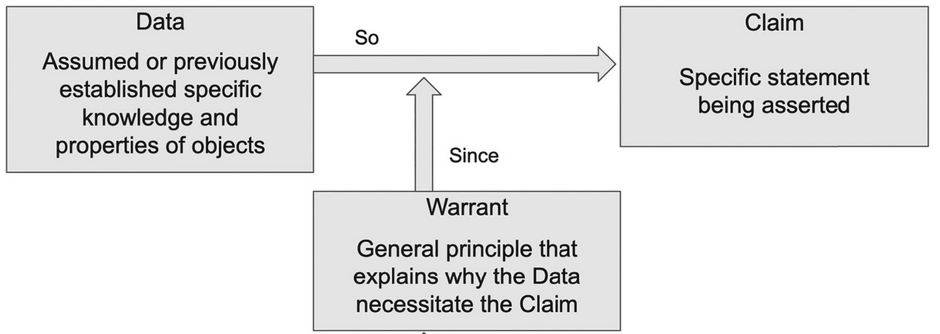
\includegraphics[width=0.5\textwidth]{../images/toulmin.png}
    \end{center}
    Helpful note: a warrant is a general principle and a data is a specific thing. For example, the group $G$ that we're thinking about is a data, and the statement ``group elements have inverses'' is a warrant.
\end{problem}


\subsection*{Subgroups of specific groups}

\begin{problem}\label{A4}
    Construct the subgroup lattice for $A_4$. Remember, this is the set of all the even permutations in $S_4$, so it consists of the following 12 elements:
    \begin{align*}
        0\text{-cycles: } &  () \\
        3\text{-cycles: } &  (1\; 2\; 3), (1\; 3\; 2), (1\; 2\; 4), (1\; 4\; 2),\\
        & (1\; 3\; 4), (1\; 4\; 3), (2\; 3\; 4), (2\; 4\; 3)\\
        \text{Double transpositions: } & (1\; 2)(3\; 4), (1\;3)(2\; 4), (1\; 4)(2\; 3)
    \end{align*}
    Here are two Cayley diagrams for $A_4$ with slightly different generating sets. I am including them in case they're helpful but mostly because I just think they're neat. The yellow node is the identity.
    \definecolor{amethyst}{HTML}{6600FF} % Close to goodnotes 
    \definecolor{lightgrey}{rgb}{.85, .85, .85}
    \colorlet{tyellow}{yellow!60!white}    
    \tikzstyle{v-tiny} = [circle, draw, fill=lightgrey,inner sep=0pt,
        minimum size=3mm]
    \tikzstyle{v-yel} = [circle, draw,
        fill=tyellow,inner sep=0pt, minimum size=3mm]
    \tikzset{p/.style={draw, very thick, amethyst, -stealth}} % Purple -->
    \[
    \begin{tikzpicture}[scale=.8,auto]
        \begin{scope}[shift={(0,0)}]
            \node (l1) at (0,2.25) [v-tiny] {};
            \node (l2) at (.866,3.75) [v-tiny] {};
            \node (l3) at (-.866,3.75) [v-tiny] {};
            \node (t1) at (0,1) [v-yel] {};
            \node (t2) at (.866,-.5) [v-tiny] {};
            \node (t3) at (-.866,-.5) [v-tiny] {};
            \node (r1) at (-3.68,-1.125) [v-tiny] {};
            \node (r2) at (-2.814,-2.5) [v-tiny] {};
            \node (r3) at (-1.948,-1.125) [v-tiny] {};
            \node (m2) at (1.948,-1.125) [v-tiny] {};
            \node (m1) at (3.68,-1.125) [v-tiny] {};
            \node (m3) at (2.814,-2.5) [v-tiny] {};
            \draw [bb] (l2) to (m1);
            \draw [bb] (m2) to (t2);
            \draw [bb] (r2) to (m3);
            \draw [bb] (l1) to (t1);
            \draw [bb] (l3) to (r1);
            \draw [bb] (r3) to (t3);
            \draw [r,decorate] (l1) to (l2);
            \draw [r] (l2) to (l3);
            \draw [r] (l3) to (l1);
            \draw [r] (t1) to (t3);
            \draw [r] (t2) to (t1);
            \draw [r] (t3) to (t2);
            \draw [r] (r1) to (r2);
            \draw [r] (r2) to (r3);
            \draw [r] (r3) to (r1);
            \draw [r] (m1) to (m2);
            \draw [r] (m2) to (m3);
            \draw [r] (m3) to (m1);
            \node at (0,-3) {$A_4=\big\<{\color{Red}(123)},{\color{eBlue}(12)(34)}\big\>$};
        \end{scope}
        %%
        \begin{scope}[shift={(10,.6)},scale=1.1]
            \node (a2) at (-45:1) [v-tiny] {};
            \node (a4) at (-135:1) [v-tiny] {};
            \node (a6) at (-225:1) [v-yel] {};
            \node (a8) at (-315:1) [v-tiny] {};
            \node (b1) at (0:2) [v-tiny] {};
            \node (b3) at (-90:2) [v-tiny] {};
            \node (b5) at (-180:2) [v-tiny] {};
            \node (b7) at (-270:2) [v-tiny] {};
            \node (c2) at (-45:4) [v-tiny] {};
            \node (c4) at (-135:4) [v-tiny] {};
            \node (c6) at (-225:4) [v-tiny] {};
            \node (c8) at (-315:4) [v-tiny] {};
            \draw [r] (b1) to (a8); \draw [r] (a8) to (a2); \draw [r] (a2) to (b1);
            \draw [r] (a4) to (a6); \draw [r] (a6) to (b5); \draw [r] (b5) to (a4);
            \draw [r] (c2) to (b3); \draw [r] (b3) to (c4); \draw [r] (c4) to (c2);
            \draw [r] (c6) to (b7); \draw [r] (b7) to (c8); \draw [r] (c8) to (c6);
            \draw [p] (b1) to (c2); \draw [p] (c2) to (c8); \draw [p] (c8) to (b1);
            \draw [p] (b5) to (c6); \draw [p] (c6) to (c4); \draw [p] (c4) to (b5);
            \draw [p] (b3) to (a2); \draw [p] (a2) to (a4); \draw [p] (a4) to (b3);
            \draw [p] (a6) to (a8); \draw [p] (a8) to (b7); \draw [p] (b7) to (a6);
            \node at (270:3.25) {$A_4 = \big\<{\color{Red}(123)},{\color{amethyst}(234)}\big\>$};
        \end{scope}
    \end{tikzpicture}
    \]
    Notes:
    \begin{itemize}
        \item Why are 3-cycles even permutations, you ask? Note that for instance $(1\; 2\; 3) = (1\;2)(1\;3)$.
        \item Please use the permutation calculator or this will take forever. Make sure left-to-right.
        \item Start by finding all the cyclic subgroups. Then ``build up.''        
        \item I guarantee that all the subgroups will have order 1, 2, 3, 4, 6, or 12. (But I won't guarantee that there's subgroups of all those orders.)
    \end{itemize}
\end{problem}

\begin{problem}\label{prob:nZ}
    This problem is about subgroups of an \textit{infinite} group: the integers $(\mathbb{Z},+)$. \\
    (Emphasis: we're writing this group \textit{additively}, so it's like $a+b$ rather than $ab$, you know?).
    \begin{enumerate}[label=\textrm{(\alph*)}]
        \item Show that the even integers, which we denote $2\mathbb{Z}=\{2k\mid k\in\mathbb{Z}\}$, form a subgroup of $\mathbb{Z}$.
        \item Show that the odd integers are not a subgroup of $\mathbb{Z}$.
        \item Show that all subsets of the form $n\mathbb{Z}=\{nk\mid k\in\mathbb{Z}\}$ for $n\in\mathbb{Z}$ are subgroups of $\mathbb{Z}$.
        \item\label{prob:nZothers} Are there any other subgroups besides the ones listed in part (c)?  Explain your answer.
        \item For $n\in \mathbb{Z}$, write the subgroup $n\mathbb{Z}$ in the ``generated by" notation.  That is, find a set $S$ such that $\langle S\rangle =n\mathbb{Z}$. (Maybe $S$ is just one element.)  Can you find more than one way to do it?
        \item Reflect on any different vibes in this infinite situation as opposed to the finite groups we've been working in so far. Did you have to adapt your strategies at all?
    \end{enumerate}
\end{problem}

\subsection*{Centers of nonabelian groups}
The center of an abelian group is boring: it is the whole group. The center of a non-abelian group is interesting: in some way, $Z(G)$ is a measurement of how non-abelian the group is. A cool thing about subgroup lattices is that they help us think about what $Z(G)$ is: since $Z(G) \leq G$, it must be one of the guys in the subgroup lattice.

\begin{problem}
    Locate $Z(G)$ in the subgroup lattice of at least one, and maybe all, of these non-abelian groups. Refer to the slides, previous homeworks, and/or Group Explorer if you need reminders of how the operation works in each of these groups.
\[
\begin{tikzpicture}[scale=1.5]
    %%
    %% Subgroup lattice of D_4
    %%
    \begin{scope}[shift={(0,0)},shorten >= -2pt,shorten <= -2pt]
        \node (D4) at (0,4) {$D_4$};
        \node (r2-f) at (-1.25,3) {$\<r^2,f\>$};
        \node (r) at (0,3) {$\<r\>$};
        \node (r2-rf) at (1.25,3) {$\<r^2,rf\>$};
        \node (f) at (-2.5,2) {$\<f\>$};
        \node (r2f) at (-1.25,2) {$\<r^2f\>$};
        \node (r2) at (0,2) {$\<r^2\>$};
        \node (r3f) at (1.25,2) {$\<r^3f\>$};
        \node (rf) at (2.5,2) {$\<rf\>$};
        \node (1) at (0,1) {$\<1\>$};
        %%
        \draw (D4) to (r2-f); \draw (D4) to (r); \draw (D4) to (r2-rf);
        \draw (r2-f) to (f); \draw (r2-f) to (r2f); \draw (r2-f) to (r2);
        \draw (r2-rf) to (rf); \draw (r2-rf) to (r3f); \draw (r2-rf) to (r2);
        \draw (r2) to (r);
        \draw (r2) to (1);
        \draw (f) to (1);
        \draw (r2f) to (1); \draw (r3f) to (1); \draw (rf) to (1);
    \end{scope}
    %%
    %% Subgroup lattice of Q_8
    %%
    \begin{scope}[shift={(5,1)},shorten >= -2pt,shorten <= -2pt]
        \node(Q8) at (0,3) {$Q_8$};
        \node(i) at (-1,2) { $\<i\>$};
        \node(j) at (0,2) { $\<j\>$};
        \node(k) at (1,2) { $\<k\>$};
        \node(-1) at (0,1) { $\<-1\>$};
        \node(1) at (0,0) { $\left\<1\right\>$};
        \draw(1)--(-1); \draw(-1)--(i); \draw(-1)--(j); \draw(-1)--(k);
        \draw(Q8)--(i); \draw(Q8)--(j); \draw(Q8)--(k);
    \end{scope}
\end{tikzpicture}
\]
\[
\begin{tikzpicture}
    \begin{scope}[shift={(0,0)},shorten >= -2pt, shorten <= -2pt,scale=.95]
        \node(G) at (0,6) {$D_3$};
        \node(r) at (-1.75,4.5) {$\<r\>$};
        \node(e) at (0,1.5) {$\<1\>$};
        \node(f) at (.2,3.3) {$\<f\>$};
        \node(rf) at (1.55,3.3) {$\<rf\>$};
        \node(r2f) at (3,3.3) {$\<r^2\!f\>$};
        \draw(G)--(r); 
        \draw(G)--(f); 
        \draw(G)--(rf); 
        \draw(G)--(r2f); 
        \draw(r)--(e); 
        \draw(f)--(e); 
        \draw(rf)--(e); 
        \draw(r2f)--(e);
        \node at (8,5) {Challenge: $A_4$, whose lattice}; 
        \node at (8,4.5) {you drew in Problem \ref{A4}.};
    \end{scope}
\end{tikzpicture}
\]
\end{problem}

\subsection*{Preview of next week: Cosets}

When we looked for copies of $C_2$ inside of $D_3$, we noted this guy, who ``has the same shape'' as $C_2\cong\<f\>\leq D_3$ but isn't a subgroup because it doesn't include the identity. This guy is called a ``coset'' -- you can think of it as a shifted version of a subgroup.

\begin{minipage}{0.4\textwidth}
    \[\begin{tikzpicture}
    \tikzstyle{r-out} = [draw, very thick, eRed,-stealth,bend right=43]
    \tikzstyle{r-in} = [draw, very thick, eRed,-stealth,bend left=38]
    %%
    \tikzstyle{every node}=[font=\small]
    \draw[cosetBlue, fill=cosetBlue,rotate=120] (0:2.2) circle (.35);
    \draw[cosetBlue, fill=cosetBlue,rotate=120] (0:0.8) circle (.35);
    \draw[cosetBlue, fill=cosetBlue,rotate=120] (0.8,-.35) rectangle(2.2,.35);
    \node (e) at (0:2) [v] {$1$};
    \node (r) at (120:2) [v] {$r$};
    \node (r2) at (240:2) [v] {$r^2$};
    \node (f) at (0:1) [v] {$f$};
    \node (r2f) at (240:1) [v] {$r^2\!f$};
    \node (rf) at (120:1) [v] {$rf$};
    \draw [r-out] (e) to (r);
    \draw [r-out] (r) to (r2);
    \draw [r-out] (r2) to (e);
    \draw [r-in] (f) to (r2f);
    \draw [r-in] (r2f) to (rf);
    \draw [r-in] (rf) to (f);
    \draw [bb] (e) to (f);
    \draw [bb] (r) to (rf);
    \draw [bb] (r2) to (r2f);
\end{tikzpicture}\]
\end{minipage}
\begin{minipage}{0.6\textwidth}
\begin{itemize}
    \item Do you see any other cosets of $\<f\>$?
    \item Can you find any cosets of $\<rf\>$? \\
    (They're shaped a bit different, yeah?)
    \item How about $\<r^2f\>$?
    \item Can you find any cosets of $\<r\>$?
\end{itemize}

\end{minipage}


\end{document}

